\chapter{Описание стенда и подготовка среды}
\label{ch:stand}

\section{Виртуальные машины}

Для выполнения работы используются три виртуальные машины в VirtualBox.

\textbf{ВМ gateway} выполняет роль шлюза и DNS/DHCP-сервера.
ОС --- Ubuntu~22.04~LTS~Server. Оперативная память: 1~ГБ, диск: 20~ГБ.
Два сетевых адаптера:
\begin{itemize}
  \item \texttt{enp0s3} --- адаптер NAT (выход в Интернет);
  \item \texttt{enp0s8} --- Internal Network (\texttt{intnet}),
        IP~\texttt{\cfgGwIP/24}.
\end{itemize}
Запущены сервисы: \texttt{bind9}, \texttt{isc-dhcp-server}.

\textbf{ВМ wordpress} --- целевой сервер данной лабораторной работы.
ОС --- Ubuntu~22.04~LTS~Server. Оперативная память: 2~ГБ, диск: 20~ГБ.
Один сетевой адаптер:
\begin{itemize}
  \item \texttt{enp0s3} --- Internal Network (\texttt{intnet}),
        статический IP~\texttt{\cfgWpIP/24}, шлюз~\texttt{\cfgGwIP}.
\end{itemize}
Установленный стек: Apache2, MariaDB, PHP~8.1, WordPress.

\textbf{ВМ desktop1} --- клиентская машина.
ОС --- Ubuntu~22.04~Desktop. Оперативная память: 2~ГБ.
Один адаптер Internal Network, IP получает по DHCP от \texttt{gateway}.
Используется для проверки доступности WordPress через браузер Firefox.

% --- Скриншот: настройка адаптеров ВМ wordpress в VirtualBox ---
\begin{figure}[h]
  \centering
  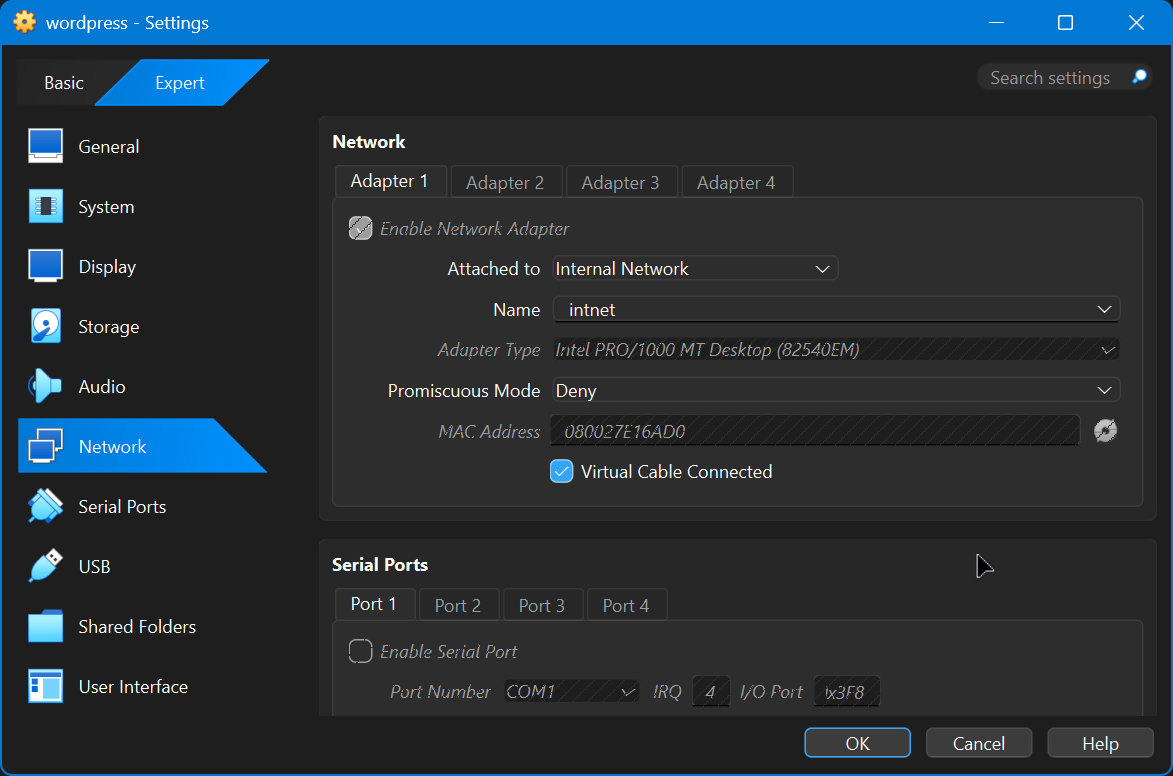
\includegraphics{img/01_vbox_wordpress_settings}
  \caption{Настройка сетевого адаптера ВМ wordpress в VirtualBox}
  \label{fig:vbox_settings}
\end{figure}

\section{Сетевая топология}

Все ВМ объединены в сеть \texttt{192.168.\cfgLabStudentN.0/24}.
Сервер \texttt{gateway} является шлюзом по умолчанию и DNS-сервером
для всей подсети.

\begin{table}[h]
  \centering
  \caption{Адресация виртуальных машин}
  \begin{tabular}{llll}
    \toprule
    ВМ & IP-адрес & Шлюз & DNS \\
    \midrule
    \texttt{gateway}   & \texttt{\cfgGwIP/24} & --- & \texttt{8.8.8.8} \\
    \texttt{wordpress} & \texttt{\cfgWpIP/24} & \texttt{\cfgGwIP} & \texttt{\cfgGwIP} \\
    \texttt{desktop1}  & DHCP & \texttt{\cfgGwIP} & \texttt{\cfgGwIP} \\
    \bottomrule
  \end{tabular}
\end{table}

\section{Добавление DNS-записи на gateway}

Перед настройкой ВМ \texttt{wordpress} на сервере \texttt{gateway}
добавляются A- и PTR-записи для нового хоста.

Запуск подготовительного скрипта:
\begin{lstlisting}
sudo bash lab8/gateway_lab8_dns.sh
\end{lstlisting}

Скрипт добавляет в прямую зону \texttt{\cfgDomain} запись:
\begin{lstlisting}
wordpress    IN  A  192.168.29.6
\end{lstlisting}
И в обратную зону:
\begin{lstlisting}
6    IN  PTR  wordpress.yazikov.iks531.local.
\end{lstlisting}

% --- Скриншот: результат gateway_lab8_dns.sh ---
\begin{figure}[h]
  \centering
  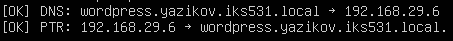
\includegraphics{img/02_gateway_dns_result}
  \caption{Результат выполнения gateway\_lab8\_dns.sh — DNS-записи добавлены}
  \label{fig:gateway_dns}
\end{figure}

\section{Подготовка ВМ wordpress}

Настройка hostname, сети и запуск скрипта подготовки выполняются
на ВМ \texttt{wordpress}:
\begin{lstlisting}
sudo bash lab8/wordpress_lab8_prepare.sh
\end{lstlisting}

Скрипт последовательно устанавливает hostname
\texttt{wordpress.\cfgDomain}, прописывает \texttt{/etc/hosts},
настраивает статический IP через Netplan, проверяет связь с gateway
и DNS, затем выполняет шаги установки стека и WordPress.

% --- Скриншот: ping до gateway и DNS ---
\begin{figure}[h]
  \centering
  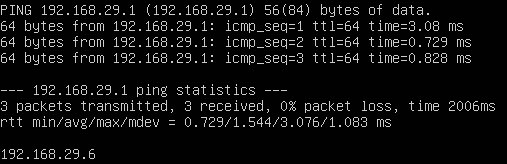
\includegraphics{img/03_wp_network_check}
  \caption{Проверка сети на ВМ wordpress: ping до gateway и DNS-резолвинг}
  \label{fig:wp_network}
\end{figure}

\endinput
